\documentclass{article}
    % General document formatting
    \usepackage[margin=0.7in]{geometry}
    \usepackage[parfill]{parskip}
    \usepackage[utf8]{inputenc}
    \usepackage{hyperref}    
    \usepackage{lineno}
    \linenumbers
    \usepackage{graphicx}
    \graphicspath{ {figures/} }
 

    \usepackage[backend=biber]{biblatex}
    \addbibresource{review.bib}

    % Related to math
    \usepackage{amsmath,amssymb,amsfonts,amsthm}
    \title{VBSCan Split17 workshop suummary}


\begin{document}

\maketitle 

\begin{center}
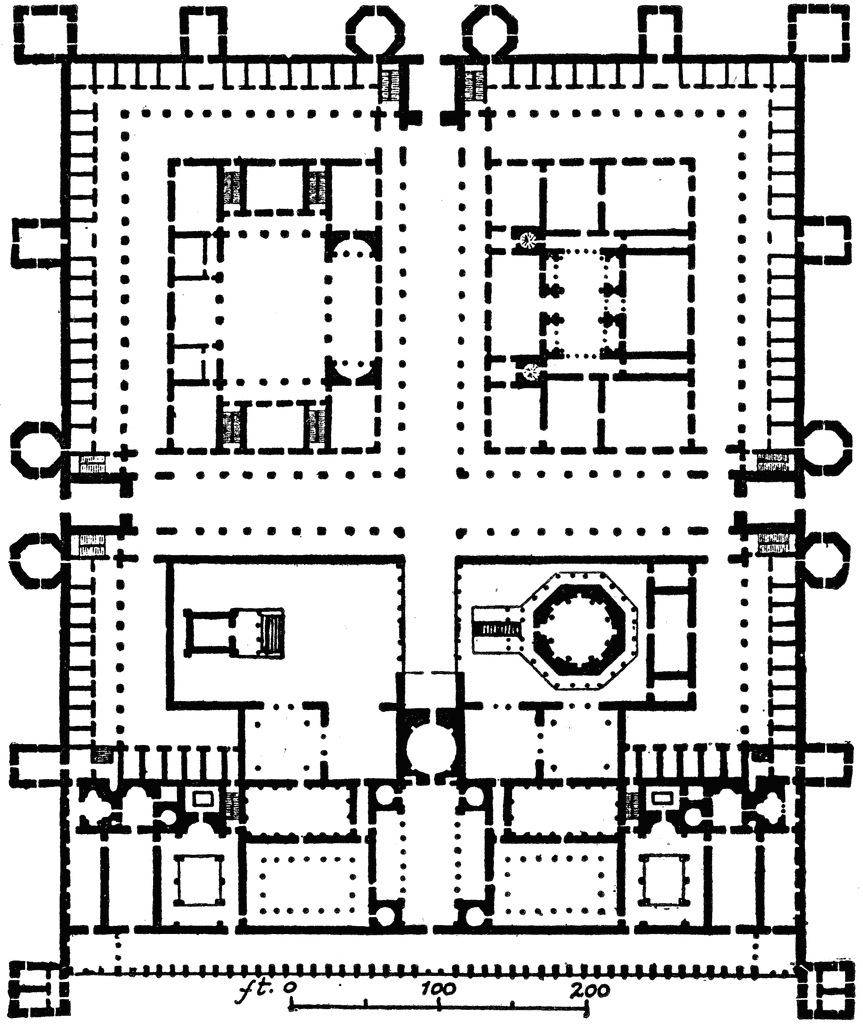
\includegraphics[scale=0.1]{palace.png}
\end{center}

\abstract{
  This document summarizes the talks and discussions happened during the VBSCan Split17 workshop,
  which is the first general meeting of the VBSCan COST Action network,
  aiming at a consistent and coordinated study of vector boson scattering
  from the phenomenological and experimental point of view, 
  for the best exploitation of the data that will be delivered by the LHC future operations.
}

\section*{Introduction}

The VBSCan COST Action Network aims at a consistent and coordinated study of vector boson scattering (VBS)
from the phenomenological and experimental point of view, 
for the best exploitation of the data that will be delivered by the LHC future operations.
The community is organized in five working groups,
three of which are dedicated to the scientific aspects of the collaboration.
One dedicated to the Theoretical Understanding of the vector boson scattering process,
which targets a detailed description of the VBS signal 
and relative backgrounds in the standard model (SM) case, 
as well as EFT modeling of BSM effects.
A second one focuses on Analysis Techniques,
studying the definition of data analysis protocols and agreements 
to maximise the significance of VBS analyses at hadron colliders, 
fostering the communication between theory and experiments.
A third one fosters the optimal deployment of VBS studies 
in the hadron collider experiments data analyses.
\newline{}
The VBSCan Network is composed by theoretical and experimental physicists from both the ATLAS and CMS experiments,
as well as data analysis experts and industrial partners.
The first general meeting of the Network happened at the end of June 2017 in Split~\cite{Ablikim:2017duf}
and was composed by reviews of the data analysis status of the art,
as well as of the theoretical and experimental instruments
relevant for VBS studies.
In this report,
a summary of the talks presented during the first general meeting of the Network is presented,
divided into sections corresponding to the Network working groups.

\section{Theoretical Understanding}
\section{Analysis Techniques}
\section{Experimental Measurements}

\section*{Conclusions}

\printbibliography

\end{document}